\documentclass[onlymath]{beamer}
\usepackage{fontspec}
\usepackage{xunicode,xltxtra}
\usepackage{polyglossia}
\usepackage{xltxtra}

\usepackage{graphicx}

\newcommand\tw\textwidth

\usefonttheme{professionalfonts}
\usetheme[secheader]{Boadilla}
\usecolortheme{whale}

\setsansfont[Mapping=tex-text]{Gill Sans Std}
\setmainlanguage{english}

\title{What Proton, Angara and Baikal have in common}
\author{Dmitry Dzhus}
\institute[BMSTU]{Moscow State Technical University n.a. N.E.Bauman}
\date{2009}

\begin{document}

\begin{frame}
  \titlepage
\end{frame}

\begin{frame}
  \frametitle{Outline}
  \tableofcontents
\end{frame}

\section{What Heavy Rockets are Used For}
\begin{frame}
  \frametitle{Launching elephants into space}

  \begin{itemize}
  \item Mankind needs heavy-class rockets
  \item Delivering large payload to low Earth orbit (LEO) \\From 160
    to 2\,000 km
  \item Launching spacecrafts to geostationary orbit (GSO)
    \\36\,000 km
  \end{itemize}
\end{frame}

\section{The Rocket Used by Russia Today}
\begin{frame}
  \frametitle{Proton}

  \begin{columns}
    \column{.2\textwidth}
    \begin{figure}
      \centering
      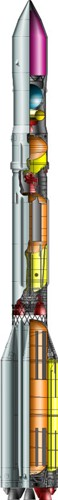
\includegraphics[scale=0.4]{Proton-K-scheme.jpg}
    \end{figure}

    \column{.8\textwidth}
    \begin{itemize}
    \item Created in the 60's at OKB-52\\ (now NPOM)
    \item Originally designed as a heavy \textsc{ICBM} capable of
      delivering a 100-megaton warhead to the United States
    \item Several modifications have been developed
    \item In service for more than 40 years
    \item Nearly 300 launches with 97\% success rate
    \end{itemize}
  \end{columns}
\end{frame}

\begin{frame}
  \frametitle{Proton achievements}
  \begin{columns}
    \column{.35\textwidth}
    \begin{figure}
      \centering
      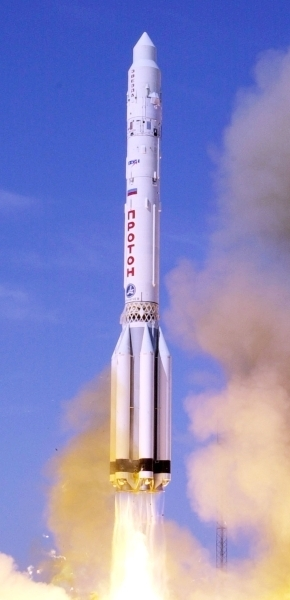
\includegraphics[scale=0.3]{Proton_Zvezda.jpg}
    \end{figure}
    \column{.65\textwidth}
    \begin{itemize}
    \item Launches of hundreds of communication and military
      satellites (since 1970)
    \item Launches of unmanned interplanetary stations\\ to Moon,
      Venus and Mars (1969--1983)
    \item Flights of Almaz and Salyut manned space stations
      (1971--1991)
    \item Delivery of modules of Mir station (1986--1996)
    \item Estiblishing of key segments of the ISS 
      on orbit (since 1998)
    \end{itemize}
  \end{columns}

\end{frame}

\begin{frame}
  \frametitle{Proton-M}
  \begin{columns}
    \column{.2\textwidth}
    \begin{figure}
      \centering
      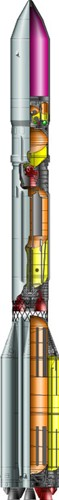
\includegraphics[scale=0.4]{Proton-M-scheme.jpg}
    \end{figure}
    
    \column{.8\textwidth}
    \begin{itemize}
    \item Modern modification of original Proton launch vehicle
      developed by Khrunichev space centre
    \item Features a new control system and Briz-M upper stage booster
    \item Capable of launching up to 22 tonnes \\to LEO and up to
      4 tonnes to GSO
    \end{itemize}
  \end{columns}

\end{frame}

\begin{frame}
  \frametitle{The evil Proton fuel}
  \begin{columns}
    \column{.45\tw}
    \begin{figure}
      \centering
      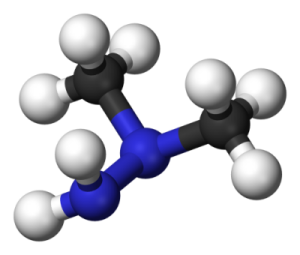
\includegraphics[scale=0.5]{UDMH.png}
    \end{figure}
    \column{.55\tw}
    \begin{itemize}
    \item Proton uses unsymmetrical dimethylhydrazine (UDMH) \\as a
      fuel, which is highly toxic
    \item Falling rocket stages pollute ground areas
    \item Ecological impact increases \\in case of launch failures
    \end{itemize}
  \end{columns}

\end{frame}

\begin{frame}
  \frametitle{Geopolitical issues}

  \begin{itemize}
  \item Proton can be launched only from Baikonur, which is a foreign
    territory (Kazakhstan)
  \item Russia pays 115 million dollars every year for rent of
    Baikonur
  \end{itemize}
\end{frame}


\section{The Rocket Planned for Future Use}
\begin{frame}
  \frametitle{Angara}
  \begin{columns}
    \column{.35\tw}
    \begin{figure}
      \centering
      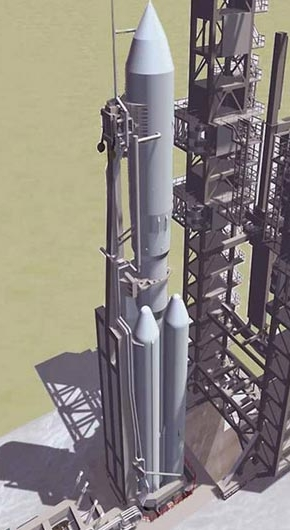
\includegraphics[scale=0.3]{Angara_Render.jpg}
    \end{figure}
    \column{.65\tw}
    \begin{itemize}
    \item A family of versatile modular launch vehicles developed by
      Khrunichev space centre
    \item No UDMH for fuel
    \item Can be launched from Plesetsk cosmodrome in northern Russia
    \end{itemize}
  \end{columns}
\end{frame}

\begin{frame}
  \frametitle{Angara modularity}
  \begin{itemize}
  \item Rocket is built from universal common core boosters (CCB)
    which are connected together
  \item Each CCB has fuel tanks and one modern RD-191 rocket engine
  \item Modular approach allows to use the same parts to produce a
    wide range of rockets, from lightweight and intermediate variants
    to heavy-duty ones
  \end{itemize}
\end{frame}

\begin{frame}
  \frametitle{Angara 1.1}
  \begin{columns}
    \column{.2\tw}
    \begin{figure}
      \centering
      
\includegraphics[scale=0.4]{Angara-1.1-scheme.jpg}
    \end{figure}
    \column{.8\tw}
    \begin{itemize}
    \item Kid version of Angara system
    \item Uses just one CCB and a simple upper stage booster
    \item Can deliver up to 2 tons to low Earth orbit
    \end{itemize}
  \end{columns}
\end{frame}

\begin{frame}
  \frametitle{Angara-A5}
  \begin{columns}
    \column{.2\tw}
    \begin{figure}
      \centering
      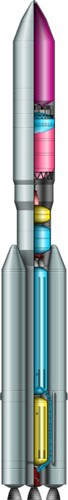
\includegraphics[scale=0.4]{Angara-A5-scheme.jpg}
    \end{figure}
    \column{.8\tw}
    \begin{itemize}
    \item The most powerful flavor of Angara
    \item Built from 5 common core boosters \\and several upper stage
      boosters
    \item Launches 24.5 tons to LEO and 4.5 tons to GSO
    \end{itemize}
  \end{columns}

\end{frame}

\begin{frame}
  \frametitle{Green rocket}
  \begin{itemize}
  \item Angara uses liquid oxygen and kerosene as a fuel
  \item No UDMH means no serious environmental damage
  \end{itemize}
\end{frame}

\begin{frame}
  \frametitle{Space Independence}
  \begin{itemize}
  \item Plesetsk is planned to become a primary launch base for Angara
    rockets
  \item Angara system will secure Russia's independent access to space
    regardless of any trends in foreign relations
  \item Facilities for Angara launches will be built at Baikonur, too
  \end{itemize}
\end{frame}

\begin{frame}
  \frametitle{Baikal}
  \begin{figure}
    \centering
    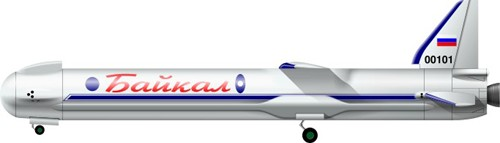
\includegraphics[scale=0.5]{Baikal.jpg}
  \end{figure}
  \begin{itemize}
  \item Shuttle booster planned for use with Angara
  \item Based on Angara's common core booster
  \item Has wings and an additional engine from MiG-29 fighter
  \item Boosts the rocket on the first stage\\ and returns back to
    ground like an airplane
  \item Utilises technologies used in Buran
  \item Can be used up to 25 times (planned 200)
  \end{itemize}
\end{frame}

\begin{frame}
  \frametitle{Baikal embrace}
  \begin{columns}
    \column{.5\tw}
    \begin{figure}
      \centering
      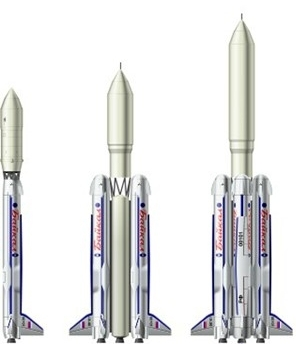
\includegraphics[scale=0.5]{Baikal-Angara.jpg}
    \end{figure}
    \column{.5\tw}
    \begin{itemize}
    \item Baikals replace one or several \\of the first stage boosters
    \item Use of shuttle boosters will allow to lower launch cost by
      25--50\%
    \item Baikal safely returns to runway instead of falling
    \end{itemize}
  \end{columns}

\end{frame}

\begin{frame}
  \frametitle{Great expectations}
  \begin{itemize}
  \item Currently Angara modules undergo testing procedures
  \item First launch is scheduled for 2011
  \item Baikal is under development but without direct government
    support (unlike Angara)
  \end{itemize}
\end{frame}

\end{document}